\documentclass[report]{article}
\usepackage{pagecolor,lipsum}
\usepackage{ragged2e}
\usepackage{graphicx}
\usepackage{subcaption}
\usepackage{enumitem}
\usepackage[none]{hyphenat}

\usepackage{tocloft}

\usepackage[norsk]{babel}
\usepackage[bottom=8em]{geometry}
\usepackage{amsmath}
\usepackage{graphicx}

\usepackage{ifluatex}
\ifluatex
%% Ved bruk av lualatex %%
\usepackage{fontspec}
\setmainfont{Linux Libertine O}
%%%%%%%%%%%%%%%%%%%%%%%%%%%
\else
%% Ved bruk av pdflatex %%
\usepackage[utf8]{inputenc}
\usepackage{libertine} % linux libertine font
%\usepackage[libertine]{newtxmath}
\usepackage[T1]{fontenc}
%%%%%%%%%%%%%%%%%%%%%%%%%%%
\fi

\usepackage{parskip}
\usepackage{xcolor}
\usepackage{lipsum}
\usepackage{calc}
\usepackage[labelfont=bf,textfont=normal,justification=justified,singlelinecheck=false,width=0.9\textwidth]{caption}

\usepackage{booktabs}
\usepackage{longtable}
\usepackage{rotating}
\usepackage{tabularx}

\usepackage{fancyhdr}


\definecolor{skde}{HTML}{0099e5}
\definecolor{skdelys}{HTML}{0099e5}
\definecolor{newcolor}{HTML}{333333}
\definecolor{number}{HTML}{D5D5D5}

%\definecolor{skde}{RGB}{0,79,158}
%\definecolor{skdelys}{RGB}{122,178,220}

\usepackage{sectsty}
\chapterfont{\color{skde}}  % sets colour of chapters
\sectionfont{\color{skde}}  % sets colour of sections
\subsectionfont{\color{skde}}  % sets colour of sections
\subsubsectionfont{\color{skde}}  % sets colour of sections

\usepackage[colorlinks, citecolor=number, linkcolor=number, urlcolor=number]{hyperref}


% Flere figurer per side etc
\renewcommand{\topfraction}{0.95}	% max fraction of floats at top
\renewcommand{\bottomfraction}{0.95}	% max fraction of floats at bottom
\renewcommand{\textfraction}{0.05}	% allow minimal text w. figs
\renewcommand{\floatpagefraction}{.8} %only pages with more than 80% of floats, will become pure float-only pages. The default is 0.6



\title{JPE\_Twitter} % tittel
\newcommand{\subtitle}{Splunk App for Twitter Mining} % undertittel
%\newcommand{\sammendrag}{Sammendrag legges inn her. \lipsum*[2]} % sammendrag
\newcommand{\sammendrag}{\justify This document was wrote, designed and made uniquely to the general understanding of JPE\_Twitter application, so it can't be edited and distribute whitout the written authorization of the author.}
\newcommand{\notatnummer}{May 2019} % dato for rapport (erstatter notatnummer)

\author{%
    Juan Alejandro P\'erez Chand\'ia \\
    Computer Engineering\\
    jalejandro.ingeniero@gmail.com\\
    %
    \vspace{1cm}
    Jocelyn Lisette Flores Scheffer\\
    English Teacher\\
    Translation Support
}

\newcommand{\hoydestrek}{125pt} % kommer an på antall forfattere

\definecolor{text}{HTML}{D5D5D5}
\definecolor{background}{HTML}{222222}

\usepackage{caption}
\usepackage[font={color=text,bf},figurename=Fig.]{caption}

	
\usepackage{geometry}
\geometry{top=2cm, bottom=2cm}
\usepackage{amsmath}
\usepackage{tikz}
\usepackage{epigraph}

\renewcommand\epigraphflush{flushright}
\renewcommand\epigraphsize{\normalsize}
\setlength\epigraphwidth{0.7\textwidth}

%\DeclareFixedFont{\titlefont}{T1}{ppl}{b}{it}{0.5in}
\DeclareFixedFont{\titlefont}{T1}{ppl}{}{}{0.5in}
\DeclareFixedFont{\subtitlefont}{T1}{ppl}{}{}{0.2in}

\makeatletter                       
\def\printauthor{%                  
    {\large \@author}}
\let\printtitle\@title
\makeatother


\newcommand\titlepagedecoration{%
\begin{tikzpicture}[overlay]%[remember picture,overlay,shorten >= -10pt]
%\draw[opacity=0.05,white, fill=skde] (-15,20) circle (125pt);
%\draw[opacity=0.15,white, fill=skde] (2,20) circle (4cm);
%\draw[opacity=0.1,white, fill=skdelys] (2,8) circle (4cm);
%\draw[opacity=0.1,white, fill=skdelys] (-10,8) circle (4cm);
%\draw[opacity=0.1,white, fill=skdelys] (2,-4) circle (4cm);
%\draw[opacity=0.05,white, fill=skde] (-15,20) circle (125pt);
\draw[opacity=0.15,white, fill=newcolor] (2,20) circle (4cm);
\draw[opacity=0.1,white, fill=newcolor] (2,8) circle (4cm);
\draw[opacity=0.1,white, fill=newcolor] (-10,8) circle (4cm);
\draw[opacity=0.1,white, fill=newcolor] (2,-4) circle (4cm);
\end{tikzpicture}%
}



\pagestyle{fancy}
 
\fancyfoot{}
\renewcommand{\footrulewidth}{0pt}
\renewcommand{\headrulewidth}{0pt}
% \fancyfoot[RO,LE]{\centering \color{text}\thepage}
\fancyfoot[R]{\centering \color{text}\thepage}
\fancyhead{}
\fancyhead[L]{}
\fancyhead[C]{}

\date{\today}




% 			S T A R T   D O C U M E N T
\begin{document}
\renewcommand*\contentsname{\color{skde}Contents}
\pagecolor{background}
\color{text}
\sloppy 

\begin{titlepage}

%\newgeometry{bottom=2cm}%, top=2cm}

\vspace*{1cm}

\noindent
{\textcolor{skde}{\titlefont \printtitle{}}}\par
%\textcolor{skde!70}{\rule{\widthof{\printtitle{}}}{10pt}}

\vspace*{0.5cm}
{\subtitlefont \subtitle}

\vspace*{1cm}
\epigraph{\sammendrag}{\notatnummer}
\null\vfill
\vspace*{1cm}
\noindent
\hfill
\begin{minipage}{0.39\linewidth}
    \begin{flushright}
        \printauthor
    \end{flushright}
\end{minipage}
%
\begin{minipage}{0.02\linewidth}
\null
\end{minipage}
\begin{minipage}{0.02\linewidth}
    \rule{1pt}{\hoydestrek}
\end{minipage}
\titlepagedecoration


\hfill

\begin{minipage}{2in}

\includegraphics[width=0.8\textwidth]{img/jp_gris}
\end{minipage}
\hfill
\begin{minipage}{3in}
\begin{flushright}
\textcolor{skde}{
\href{http://www.jpengineer.cl}{\textcolor{skde}{JPEngineer \textcopyright}}
}
\end{flushright}
\end{minipage}

%\restoregeometry

\end{titlepage}
\addtocounter{page}{1}
% \begin{large}

\section{Introduction}
JPE\_Twitter is a Splunk Application developed in Python, whose purpose is the Twitter Mining and complete integration with the log analysis tool previously mentioned. With JPE\_Twitter you can extract of Twitter important information based on words filter,
phrases, hashtag, among others and get data, that indicate what’s happening with our business or service on Twitter, building a development base to sentiment analysis on Twitter.
\newpage
\tableofcontents
\thispagestyle{empty}

\newpage
\section{Basic concepts of development}

The application is developed in Python 2.7, with the purpose of sharing Python base installation of the Splunk platform (6.x or higher) and has five essential modules:
\newline
\begin{itemize}
\item {\bf config :} The application has a configuration file called \textit{twitter.conf}, where config module can read and write the necessary parameter to the authentication with Twitter API, log files configuration, encrypt, among others.

\item {\bf security :} For the security of confidential data (authentication token), this module has what it needs to encrypt and decrypt, based on the key that the user defines in the configuration of the tokens in Splunk.

\item {\bf splunk\_read :} The purpose of this modules is take all the entered parameters from the Splunk platform and take them to the corresponding module (config, security, service, among others).

\item {\bf service :} Responsible to start, stop and restart the service, besides to obtain its status.

\item {\bf twitter :} Corresponding to the main module, who will return everything filtered on Twitter.
\newline
\end{itemize}

Besides, JPE\_Twitter has its own log files, to make process debug through Splunk or directly looking at log files: 
\newline
\begin{itemize}
\item {\bf config.log :} Show the ran process by \textit{config} module, including its problem (if there is
any).

\item {\bf service.log :} Show the service state and its PID, besides include problems that this service might have.

\item {\bf twitter.log :} Show the authentication state with Twitter API and filtered messages from this social network.

\item {\bf splunk\_read.log :} Show the ran process by \textit{splunk\_read} module, including its problem (if there is any).
\newline
\end{itemize}

\begin{figure}[h!]
	\centering
	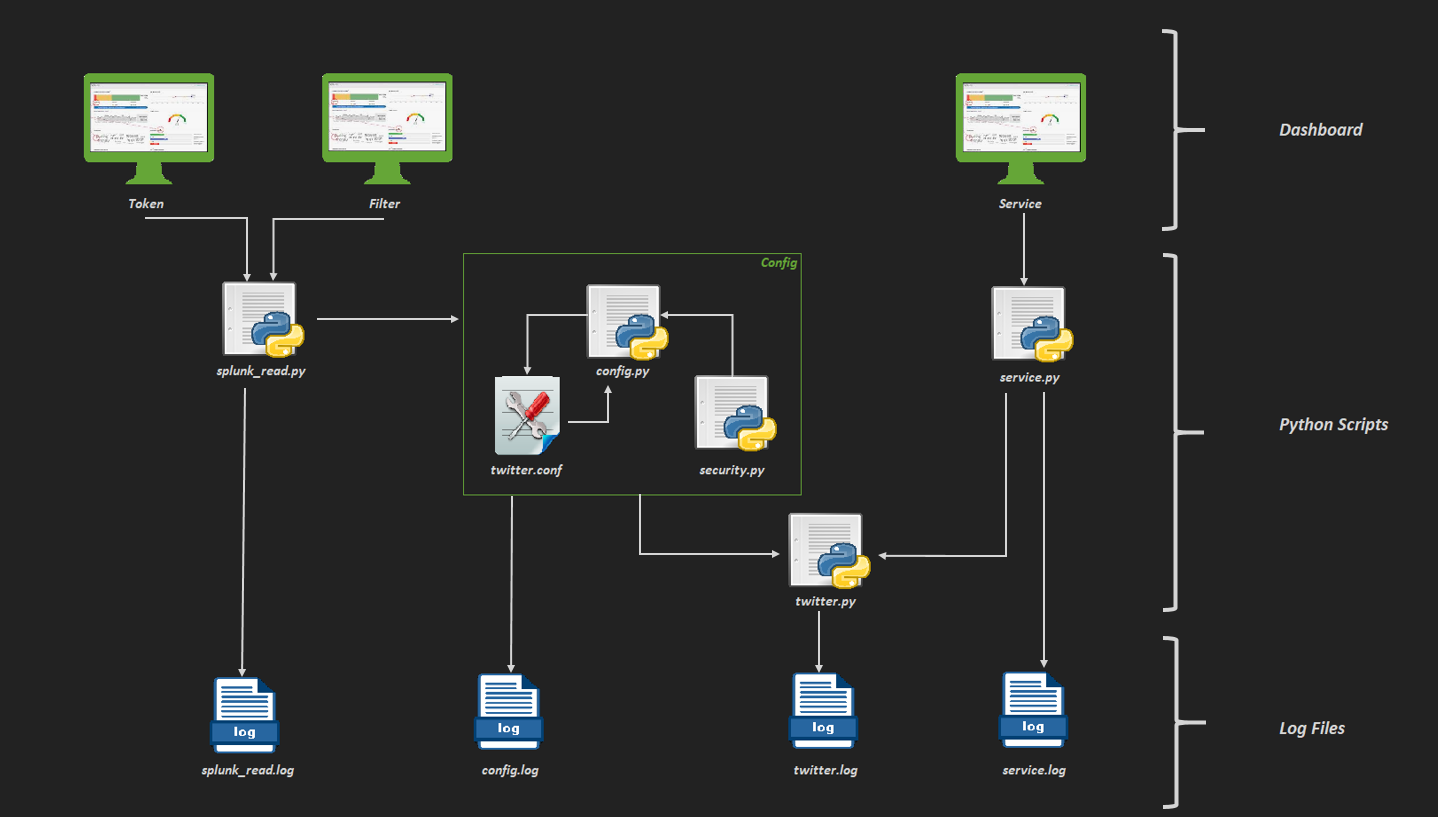
\includegraphics[scale=0.33]{img/arquitectura.PNG}
	\caption{\color{text}JPE\_Twitter General Diagram}
\end{figure}

\textit{\small \textbf{Important:} All the necessary libraries to  the proper running of the application, are included on the installation package.}
\newpage
\subsection{Dashboards}

To the administration of Twitter listening process exists three important dashboards, that allows to configure the authentication tokens and filters, also allows to start, stop and restart  the service or check its status: 
\newline
\begin{itemize}
\item Token and Security
\item Filter
\item Service
\newline
\end{itemize}

Besides, have three basic dashboards, that allows to show Twitter general information base on the filters configurated, such as user with most followers, hashtag the most used and users mention: 
\newline
\begin{itemize}
\item Twitter Users
\item Twitter Hashtag
\item Twitter Comments
\newline
\end{itemize}

\subsubsection{Token and Security}
This dashboard allows to configure the authentication of Twitter API tokens, which are: \textit{consumer key, consumer secret, access token and access secret}. This tokens are stored in the configuration file \textit{twitter.conf} and related to security, the authentication tokens can be encrypted to prevent that other people access to them, only  is necessary to write an encryption key in the same panel, after to indicate that you want to encrypt the tokens. 
\newline
\begin{figure}[h!]
	\centering
	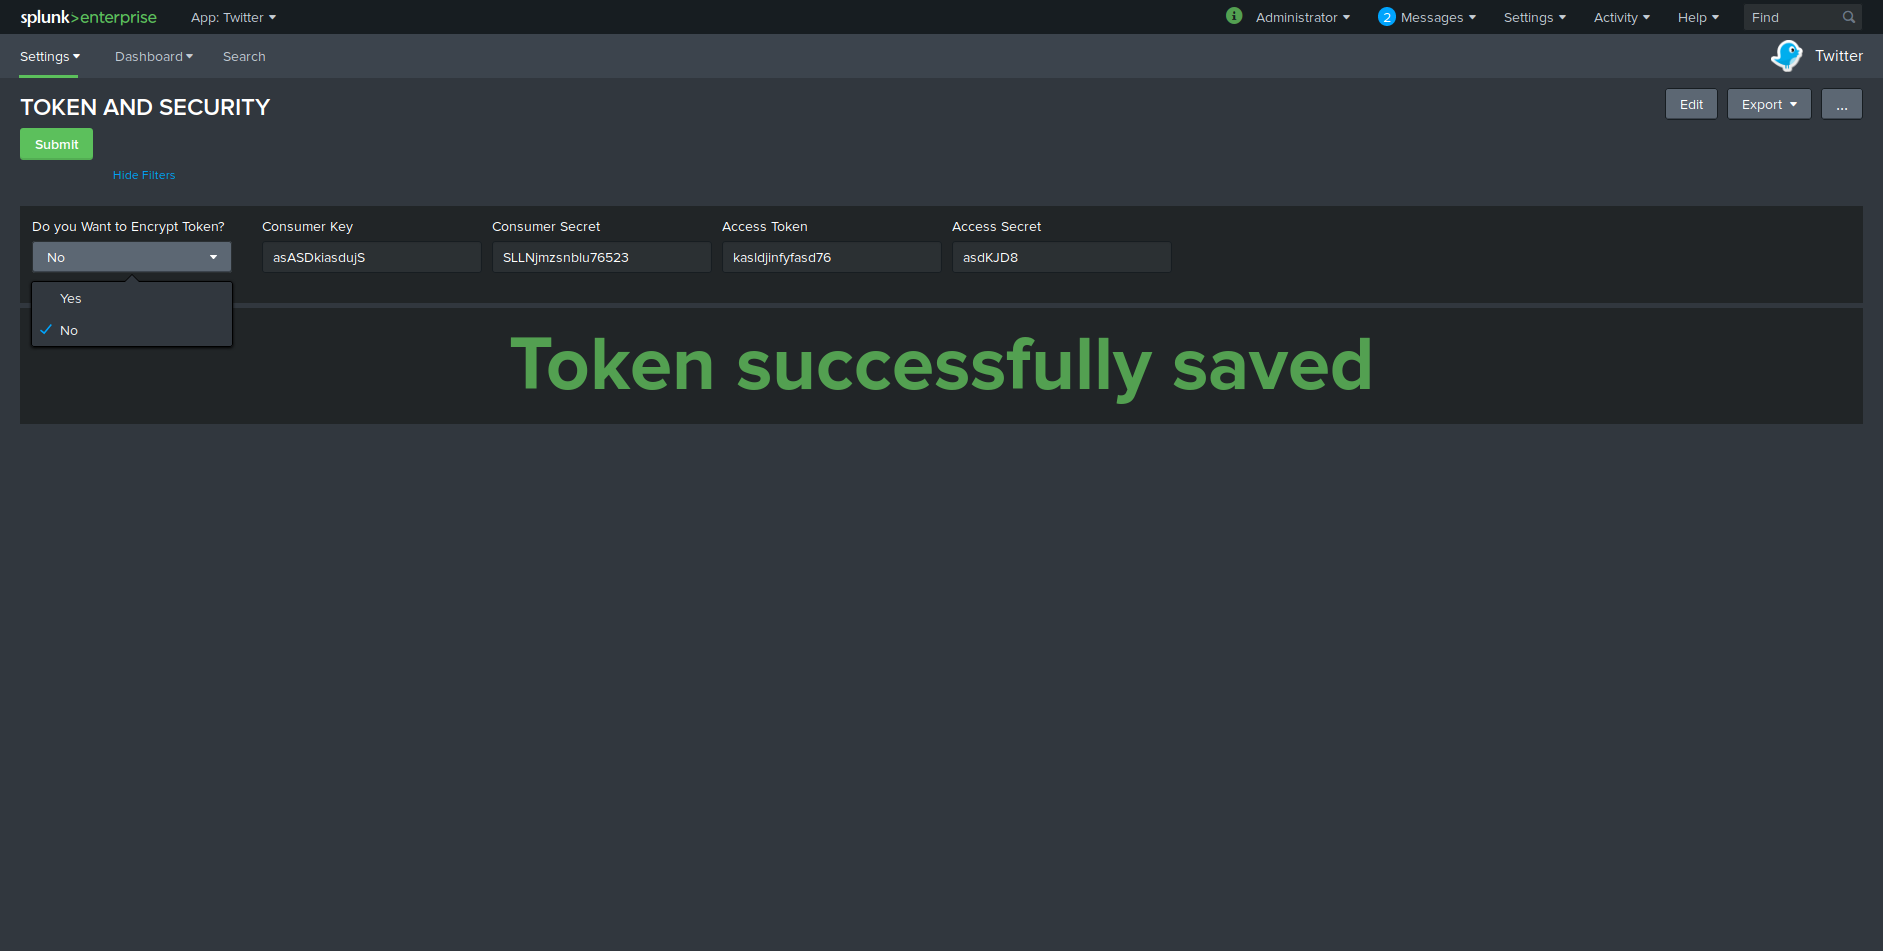
\includegraphics[scale=0.2]{img/token.png}
	\caption{\color{text}Setting: Token and Security Dashboard}
\end{figure}
\newline
It is important to consider that: to obtain tokens, you must create a developer account on Twitter (\url{https://developer.twitter.com})
\newpage
\subsubsection{Filter}

This dashboard allows to configure filters that will be apply in the listening process. Configuration option included adding a new filter to what is already configured or create a new filter, replacing the previous ones, by choosing \textit{add o new} respectively.\\
Entered filters can be words, phrases, hashtag, among others and should be separated by comma. 
\newline
\begin{figure}[h!]
	\centering
	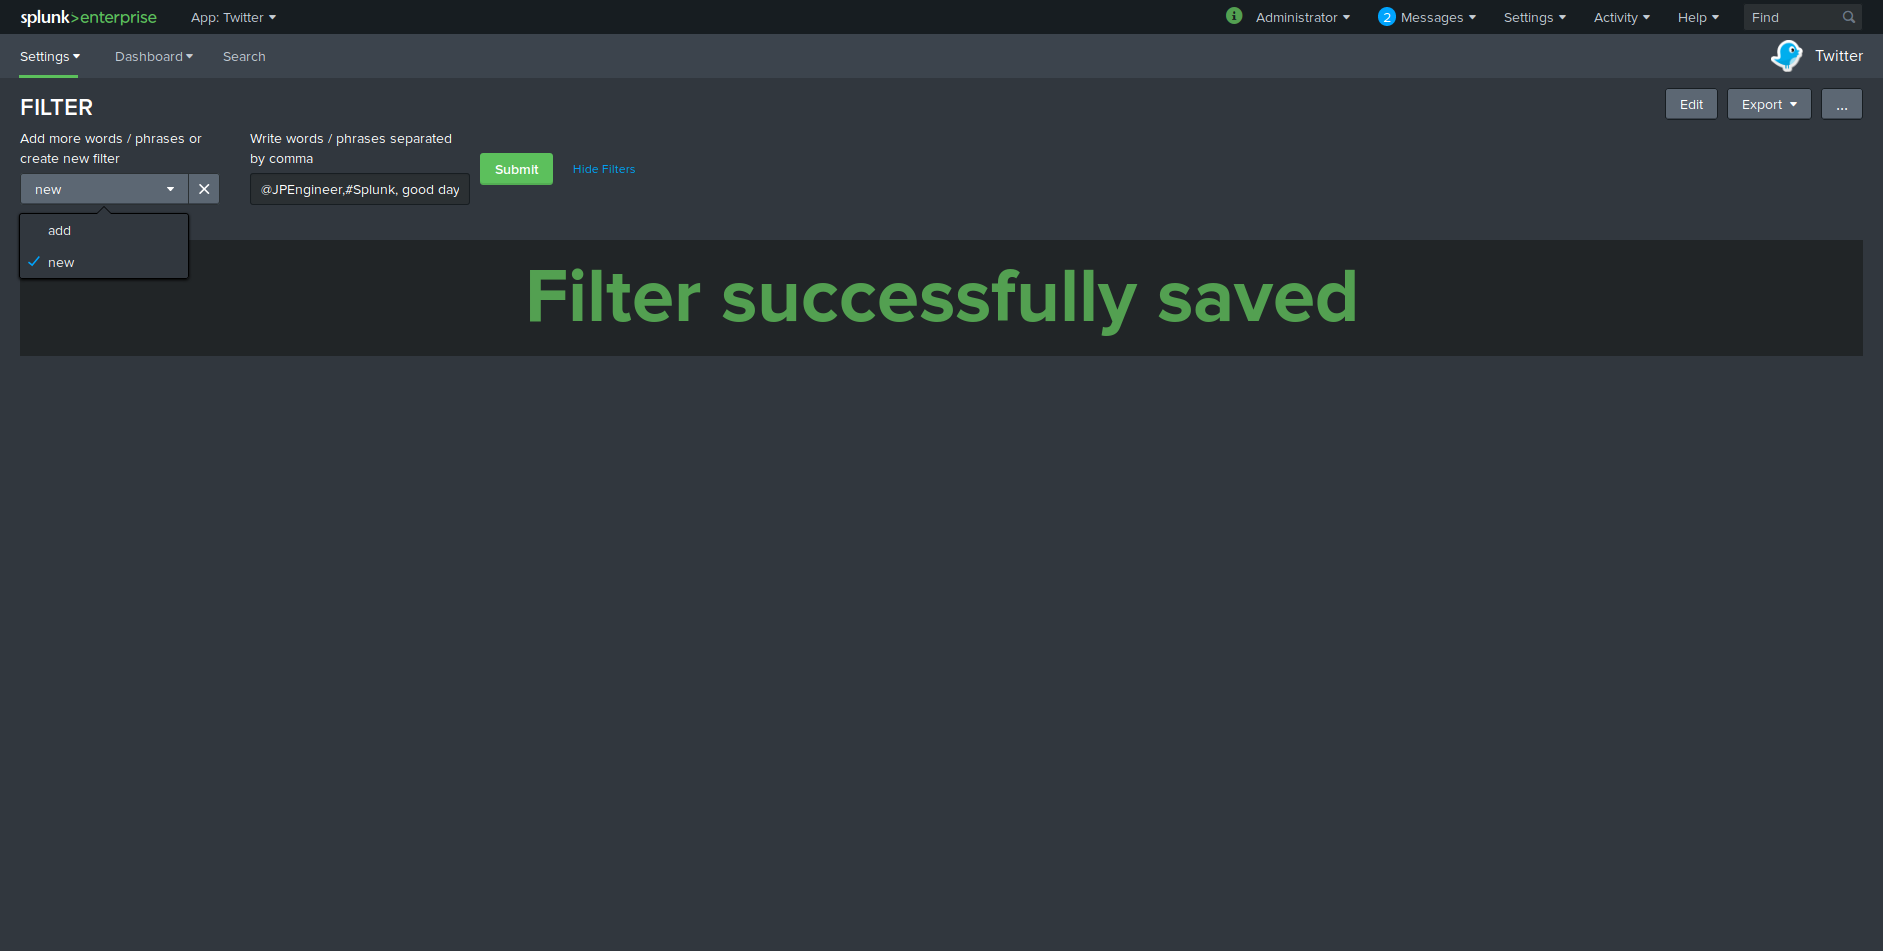
\includegraphics[scale=0.2]{img/filter.png}
	\caption{\color{text}Setting: filter Dashboard}
\end{figure}

\subsubsection{Service}
This dashboard allows  the action of run over Twitter service. Start option allows to initiate the service and begin to index the data obtained from Twitter and as previous requirement, you will need to have an authentication tokens and filters configurated. Stop option is responsible to stop the service. Restart option allows automatically to stop and start the service if it is require for own developments or other reasons. Status option shows service information (active or stopped).
\newline
\begin{figure}[h!]
	\centering
	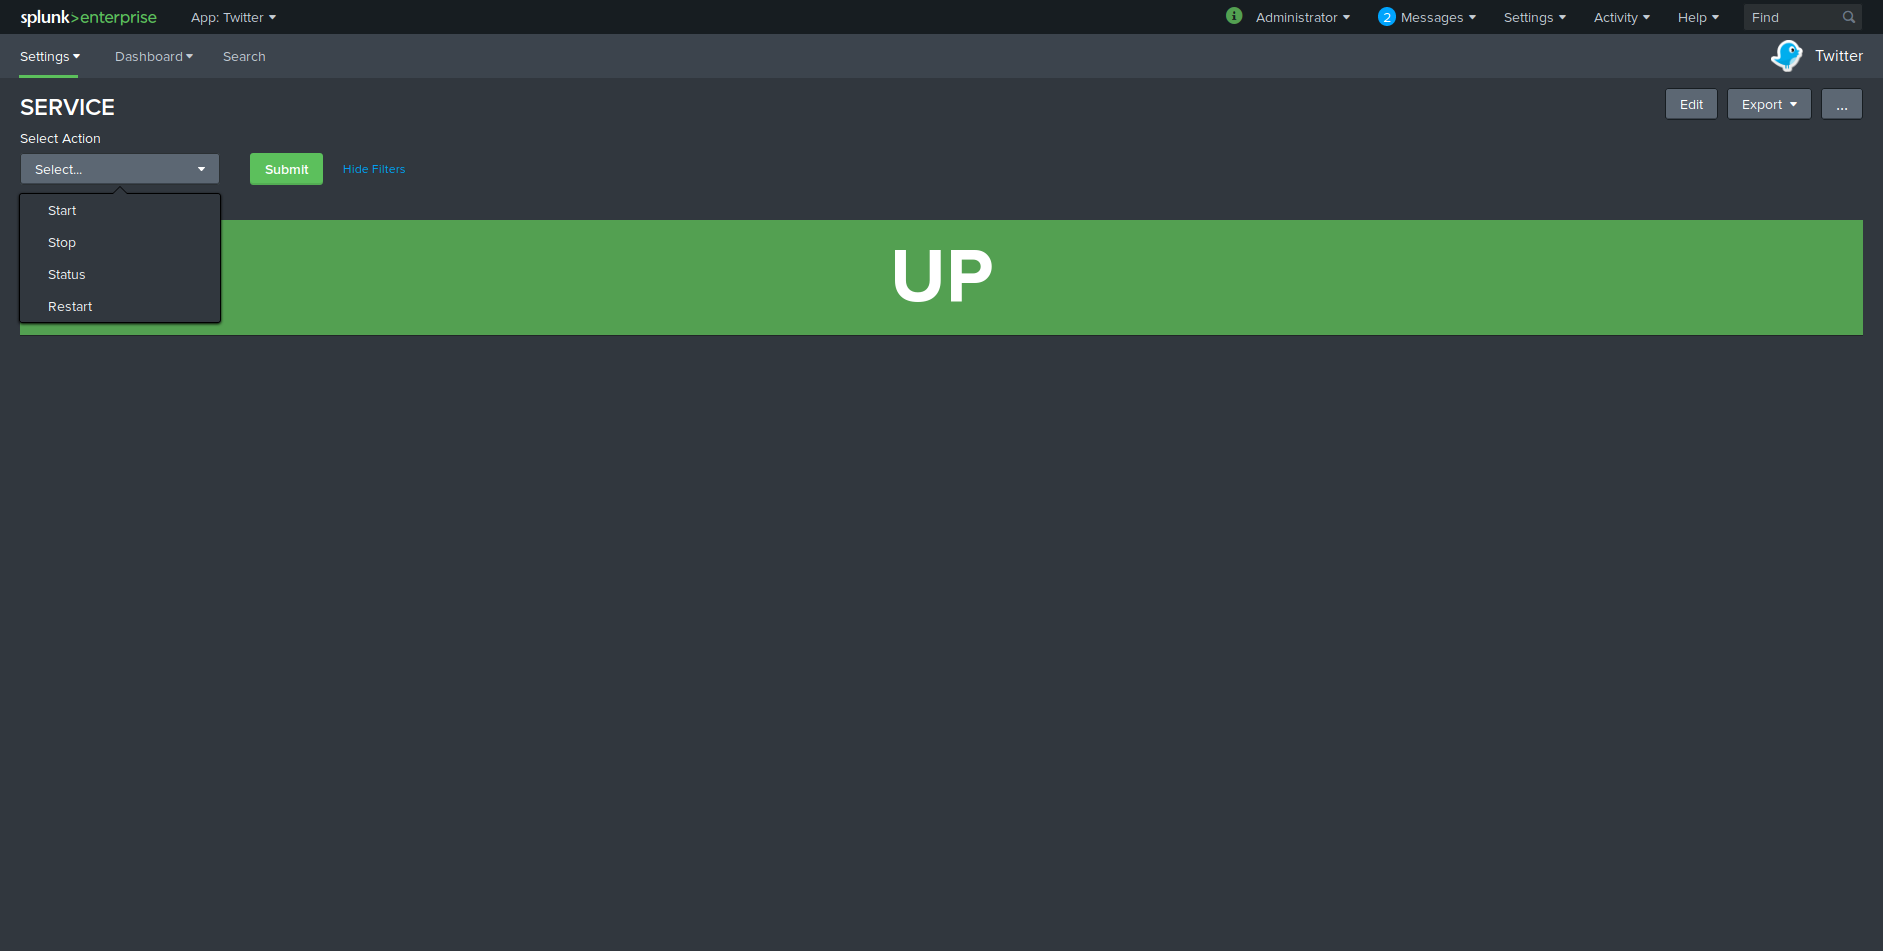
\includegraphics[scale=0.2]{img/service.png}
	\caption{\color{text}Setting: Service Dashboard}
\end{figure}


\subsubsection{Twitter Users}

This dashboard shows Twitter users information, as followers number, name, alias and location. On the same dashboard new developments can be applied to obtain additional information.
\newline
\begin{figure}[h!]
	\centering
	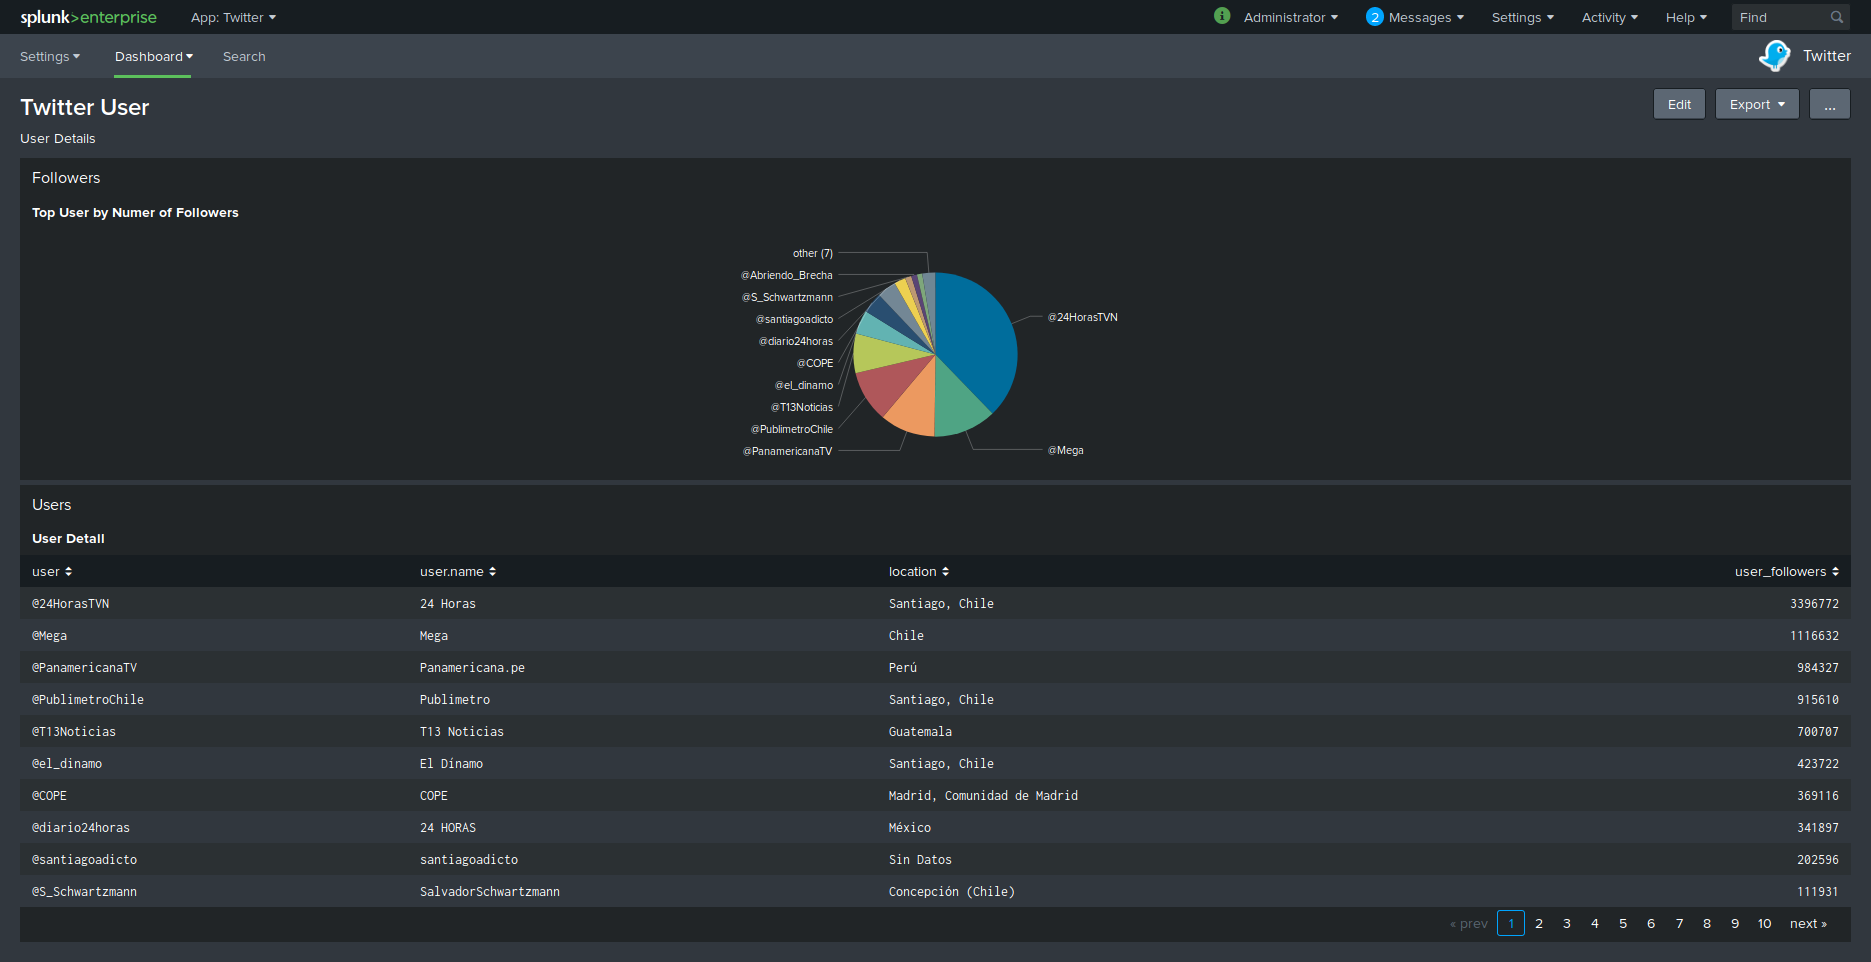
\includegraphics[scale=0.2]{img/user.png}
	\caption{\color{text}Twitter User Dashboard}
\end{figure}

\subsubsection{Twitter Hashtag}

This dashboard shows hashtag information (trending topic). On the same dashboard new developments can be applied to obtain additional information.
\newline
\begin{figure}[h!]
	\centering
	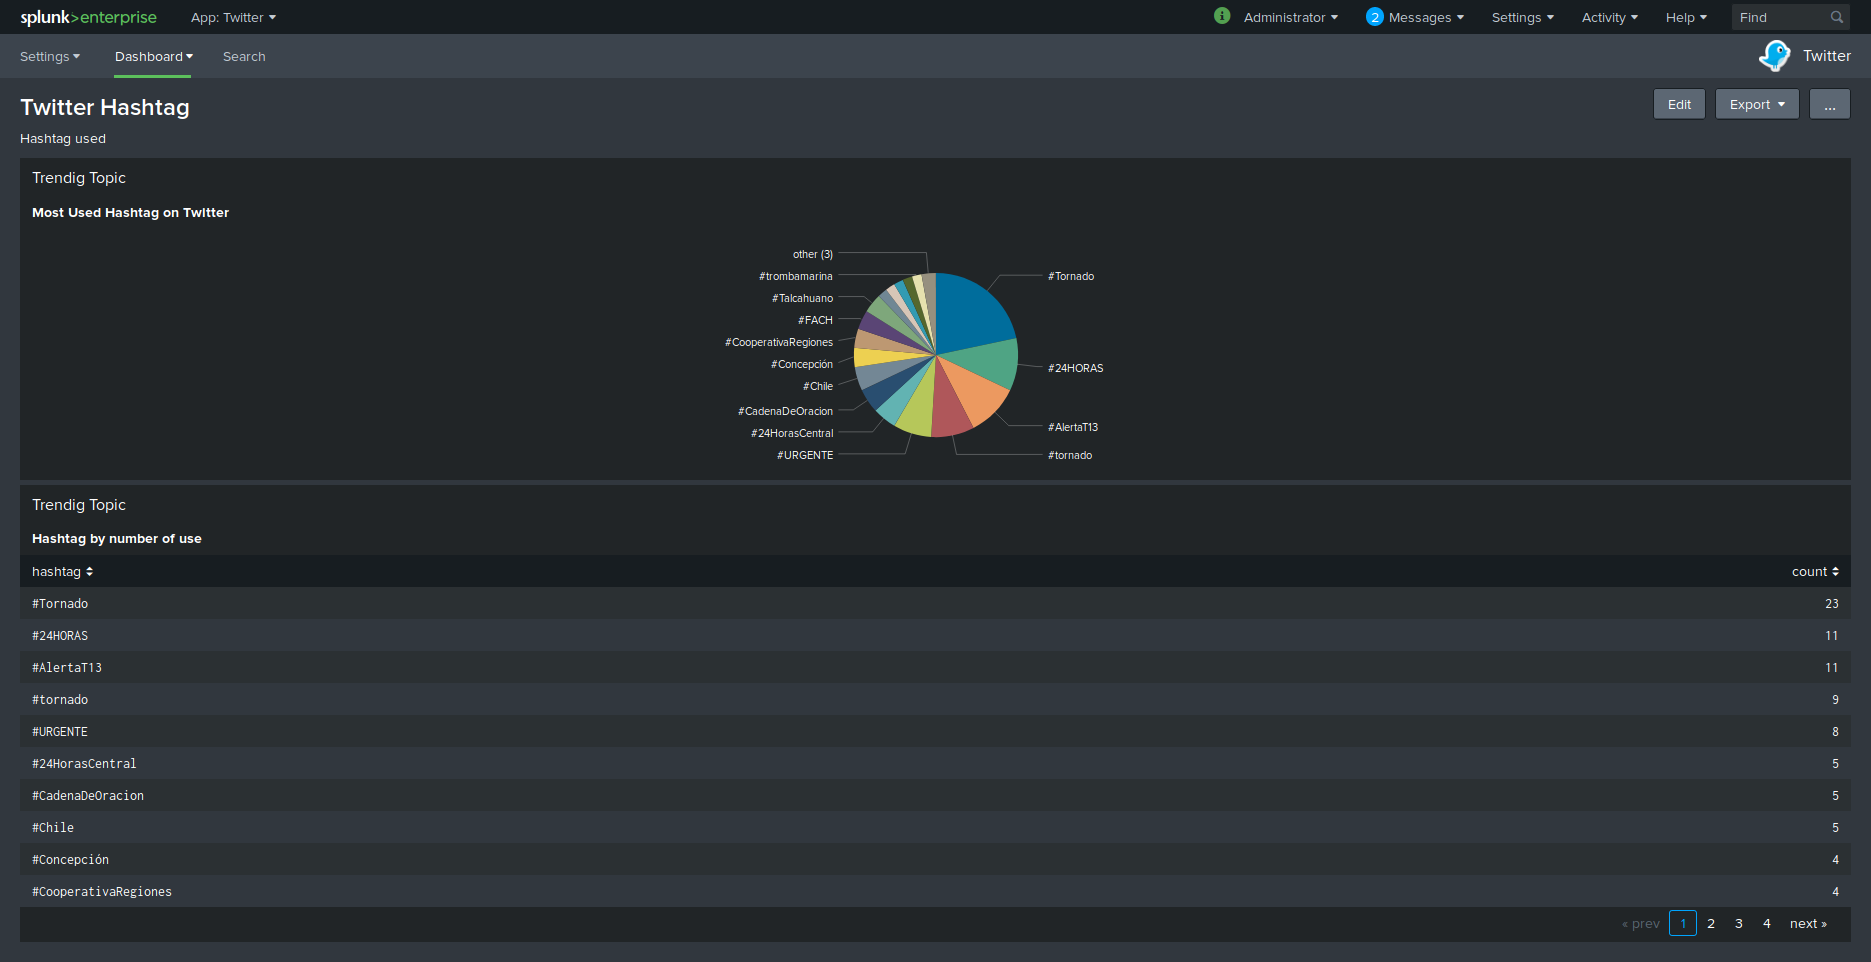
\includegraphics[scale=0.2]{img/hashtag.png}
	\caption{\color{text}Twitter Hashtag Dashboard}
\end{figure}

\newpage

\subsubsection{Twitter Comments}
This dashboard shows the details of the most commented users, comments made and user information. On the same dashboard new developments can be applied to obtain additional information.
\newline
\begin{figure}[h!]
	\centering
	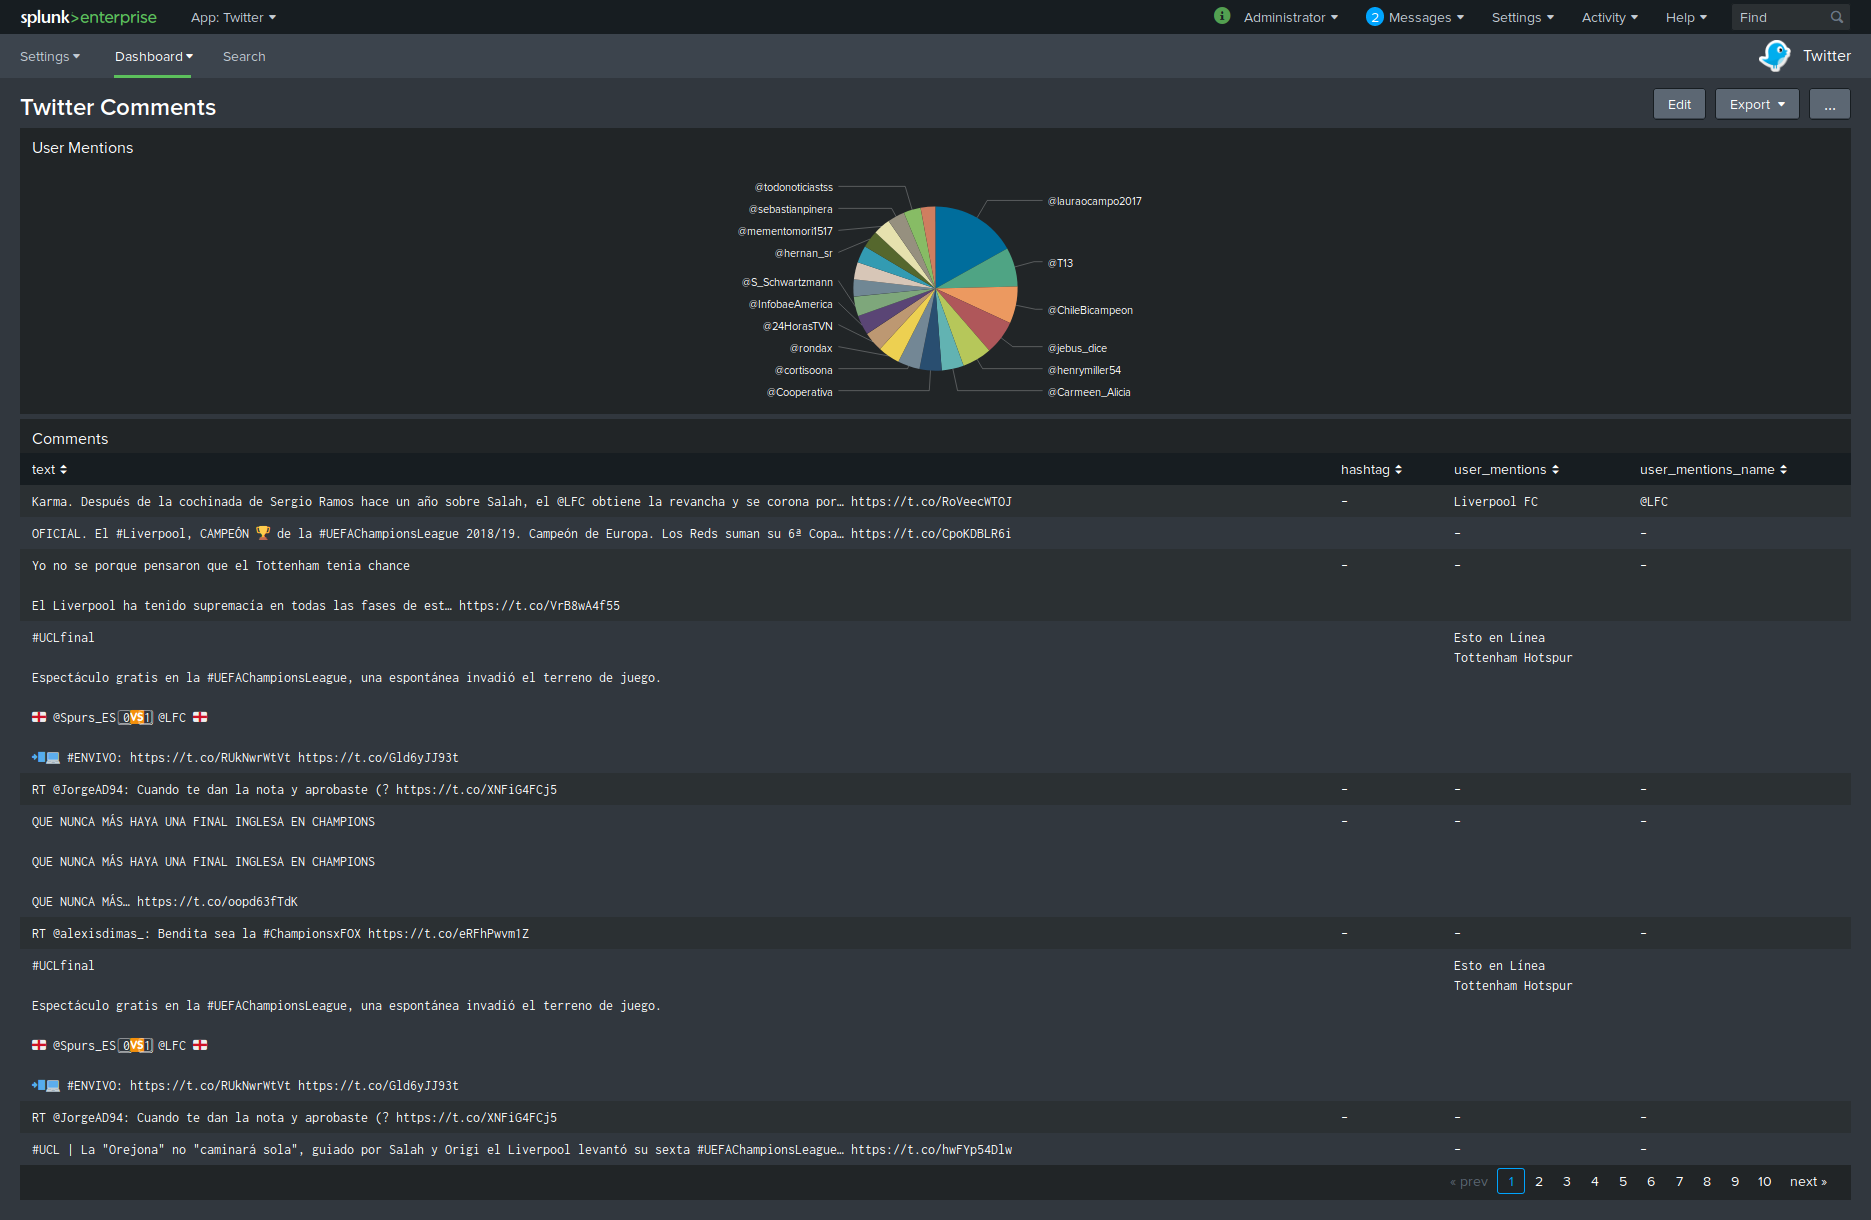
\includegraphics[scale=0.2]{img/comments.png}
	\caption{\color{text}Twitter Comments Dashboard}
\end{figure}

\newpage

\section{Installation}
 
JPE\_Twitter was tested in Splunk 6.x versions or higher and was development on Splunk 7, which will be used in the following installation guide.\\
\\
Considering that the application is downloaded, you must follow the next steps:
\newline
\begin{enumerate}[label=(\alph*)]
\item Make click on top left of the Splunk platform, says \textbf{App: Search \& Reporting} > \textbf{Manage Apps}
\item Make click on top right of the Splunk platform, on the buttom \textbf{Install Apps from File}
\item Make click on \textbf{Examine} and select JPE\_Twitter.zip, later make click on \textbf{Upload}
\newline
\end{enumerate}

\begin{figure}[h!]
  \centering
  \begin{subfigure}[b]{0.49\linewidth}
    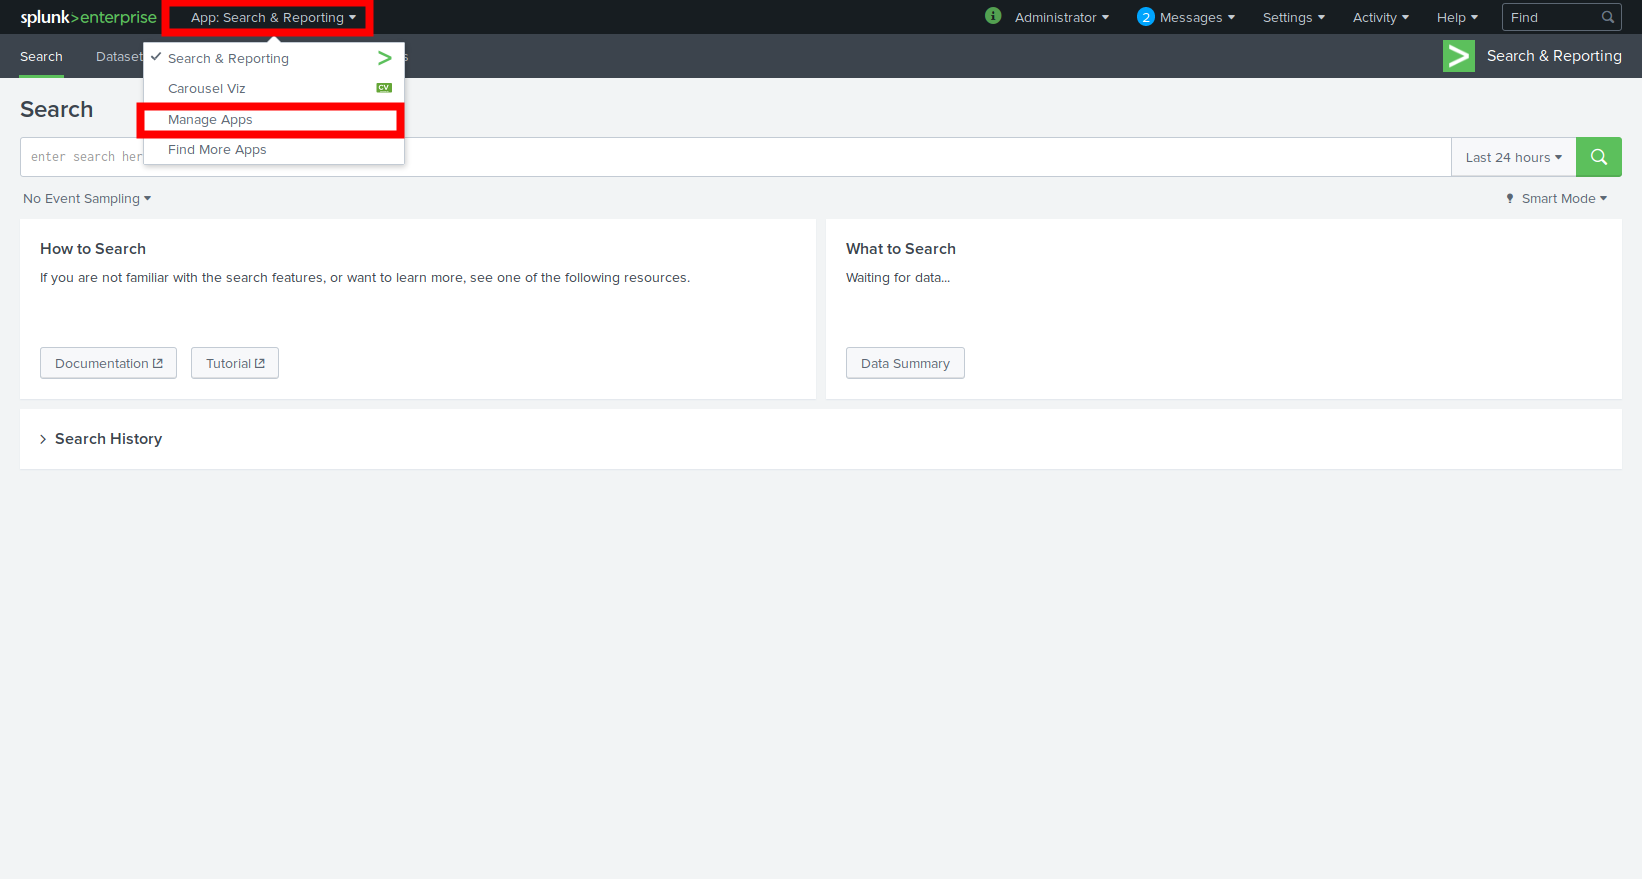
\includegraphics[width=\linewidth]{img/a.png}
     \caption{\color{text} Manage Apps}
  \end{subfigure}
  \begin{subfigure}[b]{0.49\linewidth}
    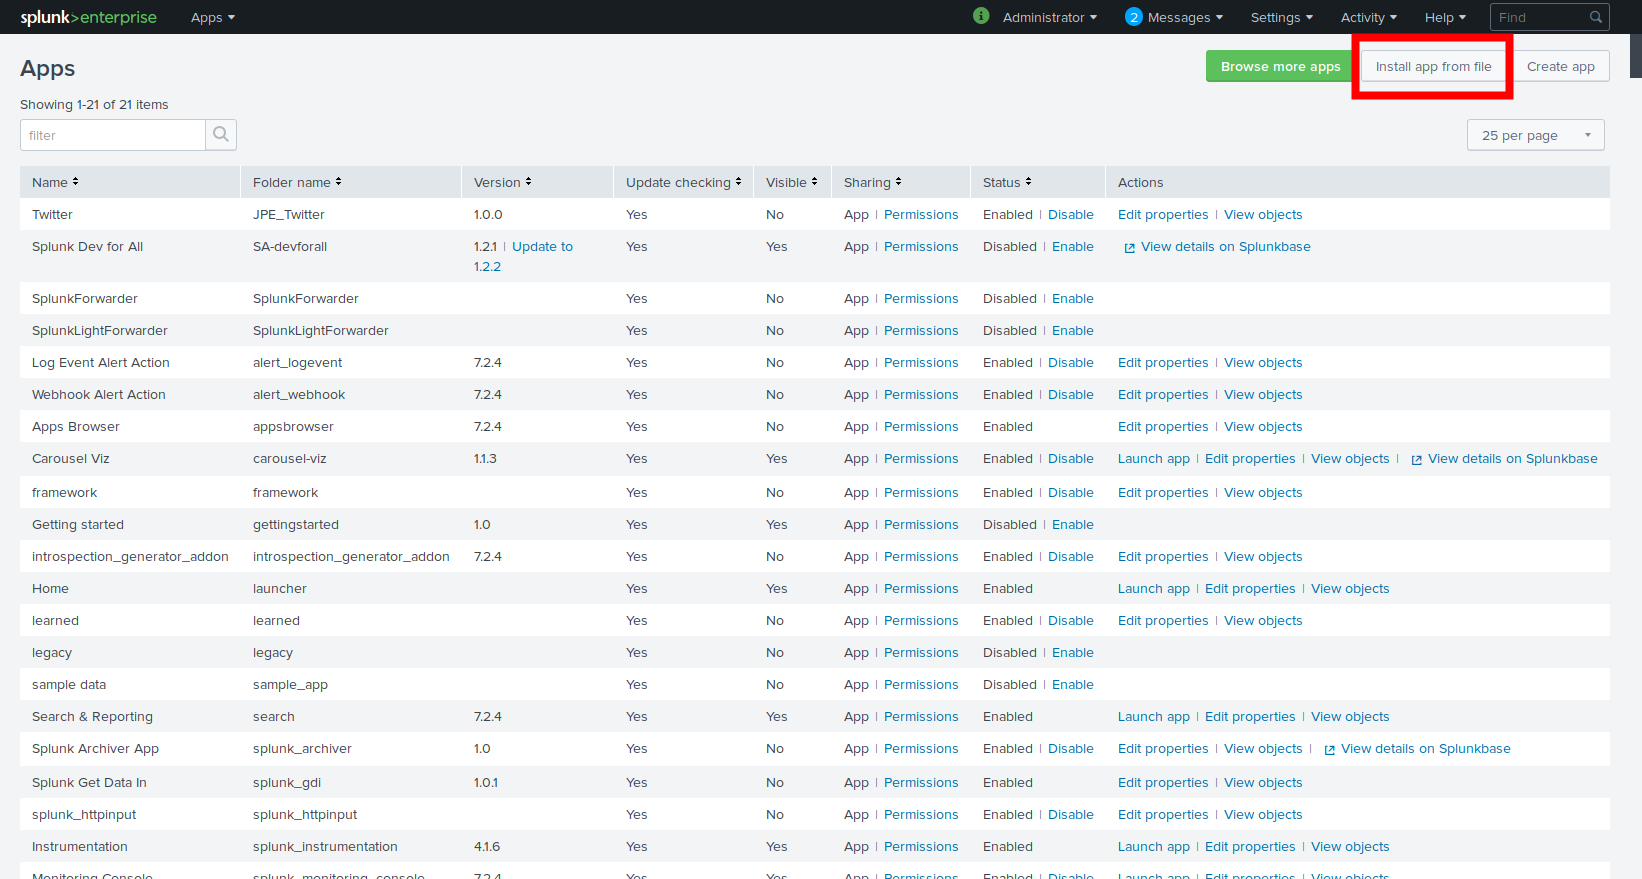
\includegraphics[width=\linewidth]{img/b.png}
    \caption{\color{text} Install Apps from File}
  \end{subfigure}
  \begin{subfigure}[b]{0.49\linewidth}
    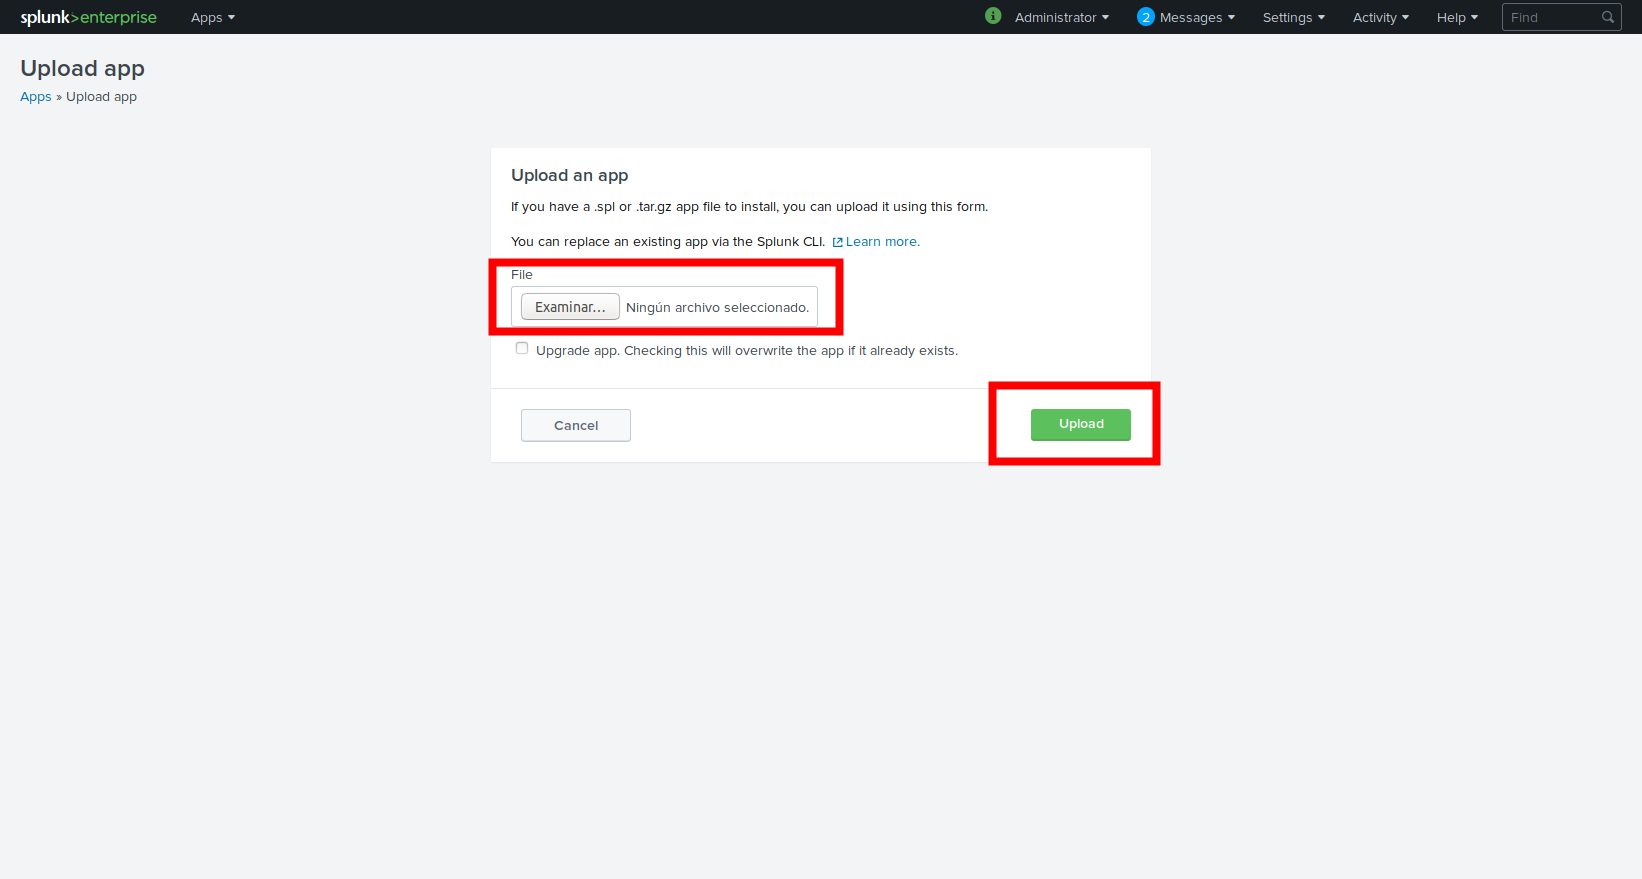
\includegraphics[width=\linewidth]{img/c.png}
    \caption{\color{text} Upload}
  \end{subfigure}
  \caption{\color{text}JPE\_Twitter Installation}
  \label{fig:instalacion}
\end{figure}
With these simple steps, JPE\_Twitter will be installed. The recomendation is to restart Splunk.
\newpage
\section{Validations}

In order to validate the installation, you must follow the next steps:
\newline

\begin{enumerate}[label=(\alph*)]
\item Make click on top right of Splunk platform, in \textbf{Setting > Indexes} section.
\item Validate that \textbf{twitter} index exist.
\item Make click on \textbf{Setting > Source Types} and validate that \textbf{twitter, setting} y \textbf{service} source types exist.
\newline
\end{enumerate}

\begin{figure}[h!]
  \centering
  \begin{subfigure}[b]{0.49\linewidth}
    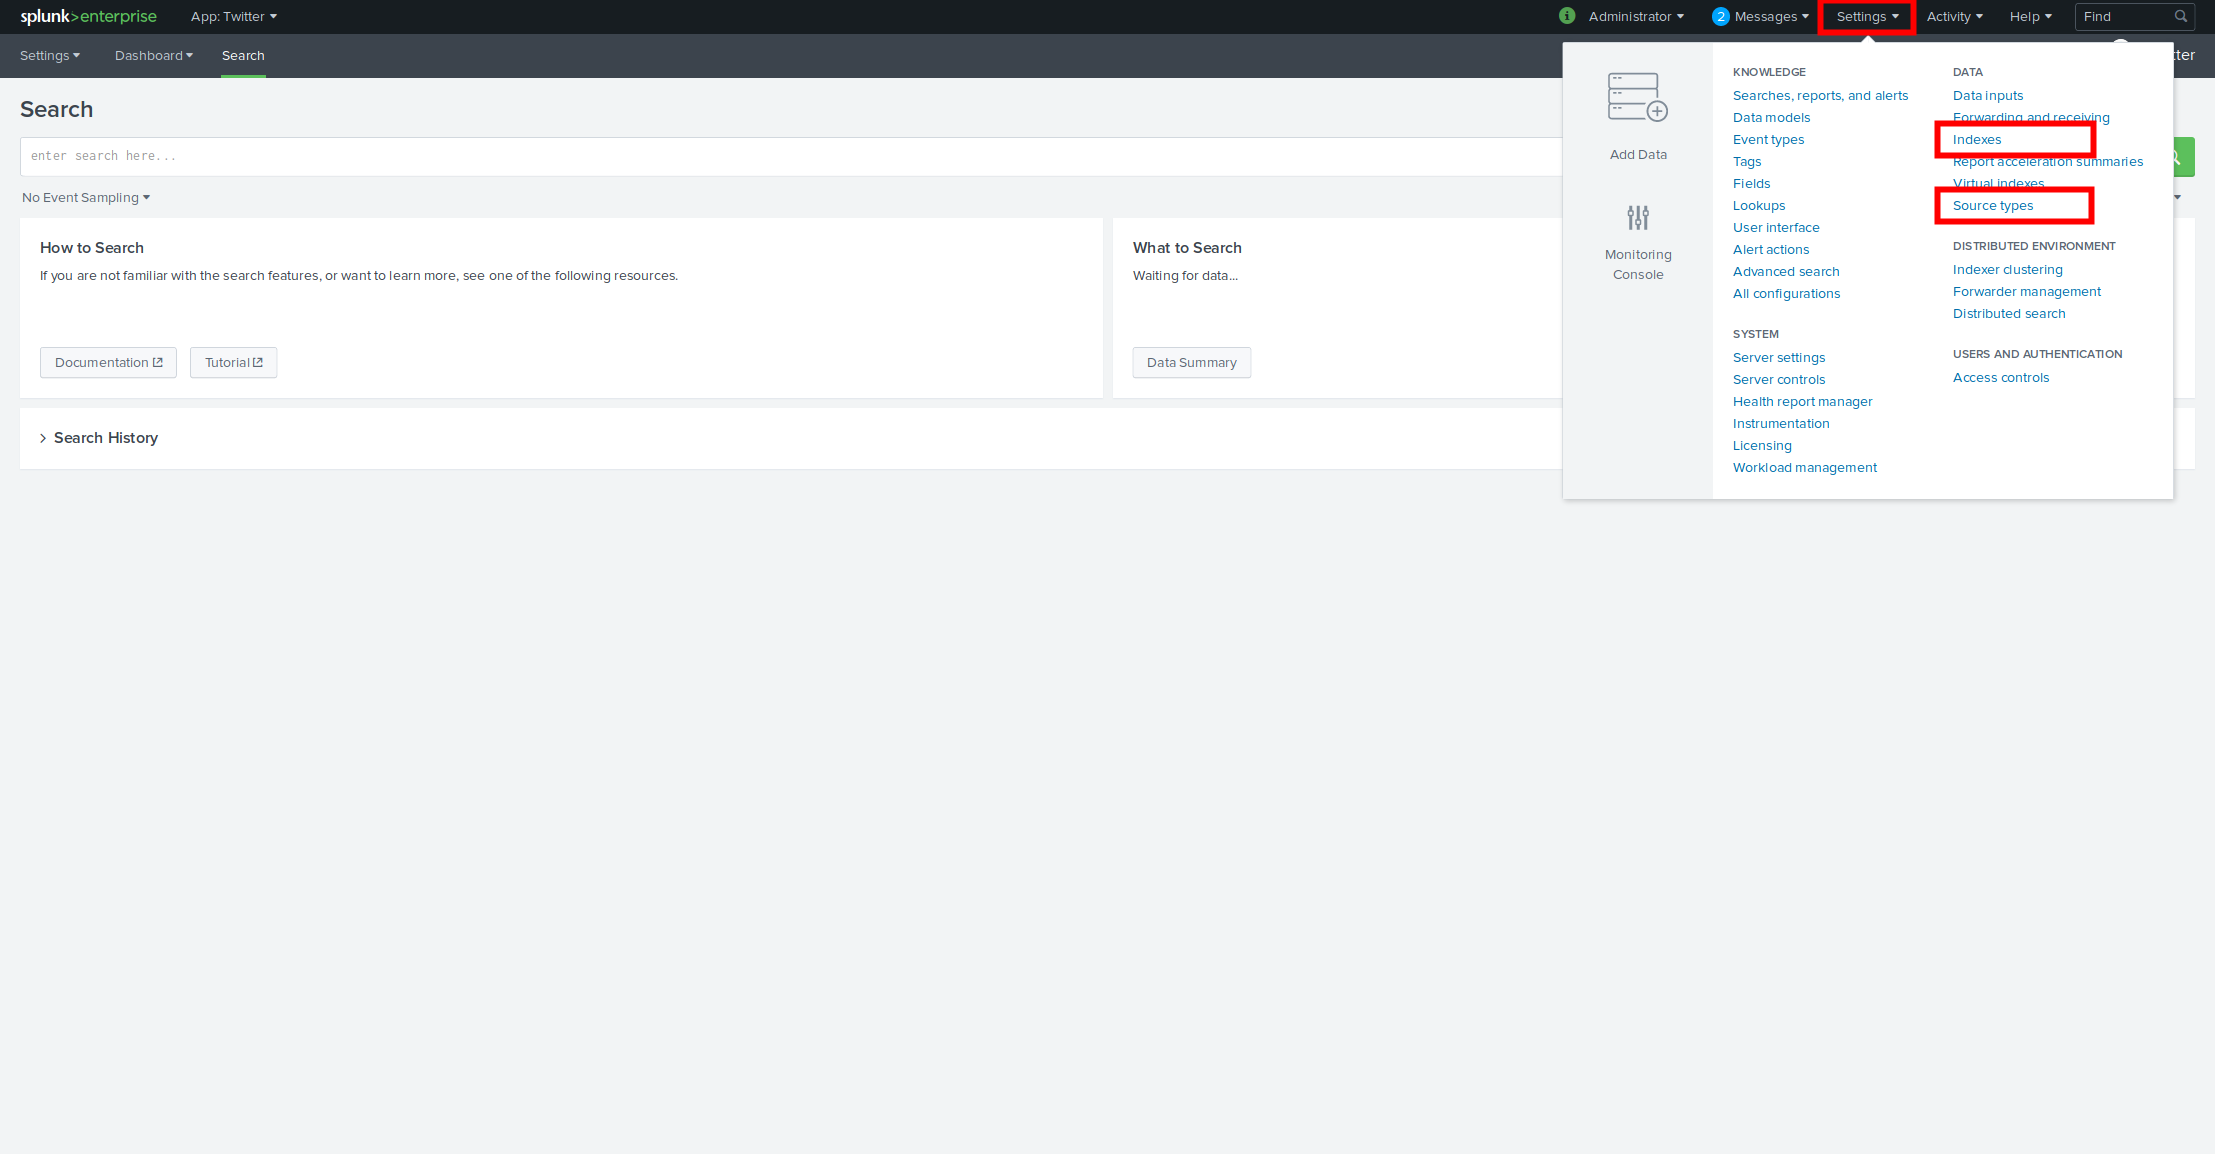
\includegraphics[width=\linewidth]{img/f.png}
     \caption{\color{text} Setting: Index - Sourcetype}
  \end{subfigure}
  \begin{subfigure}[b]{0.49\linewidth}
    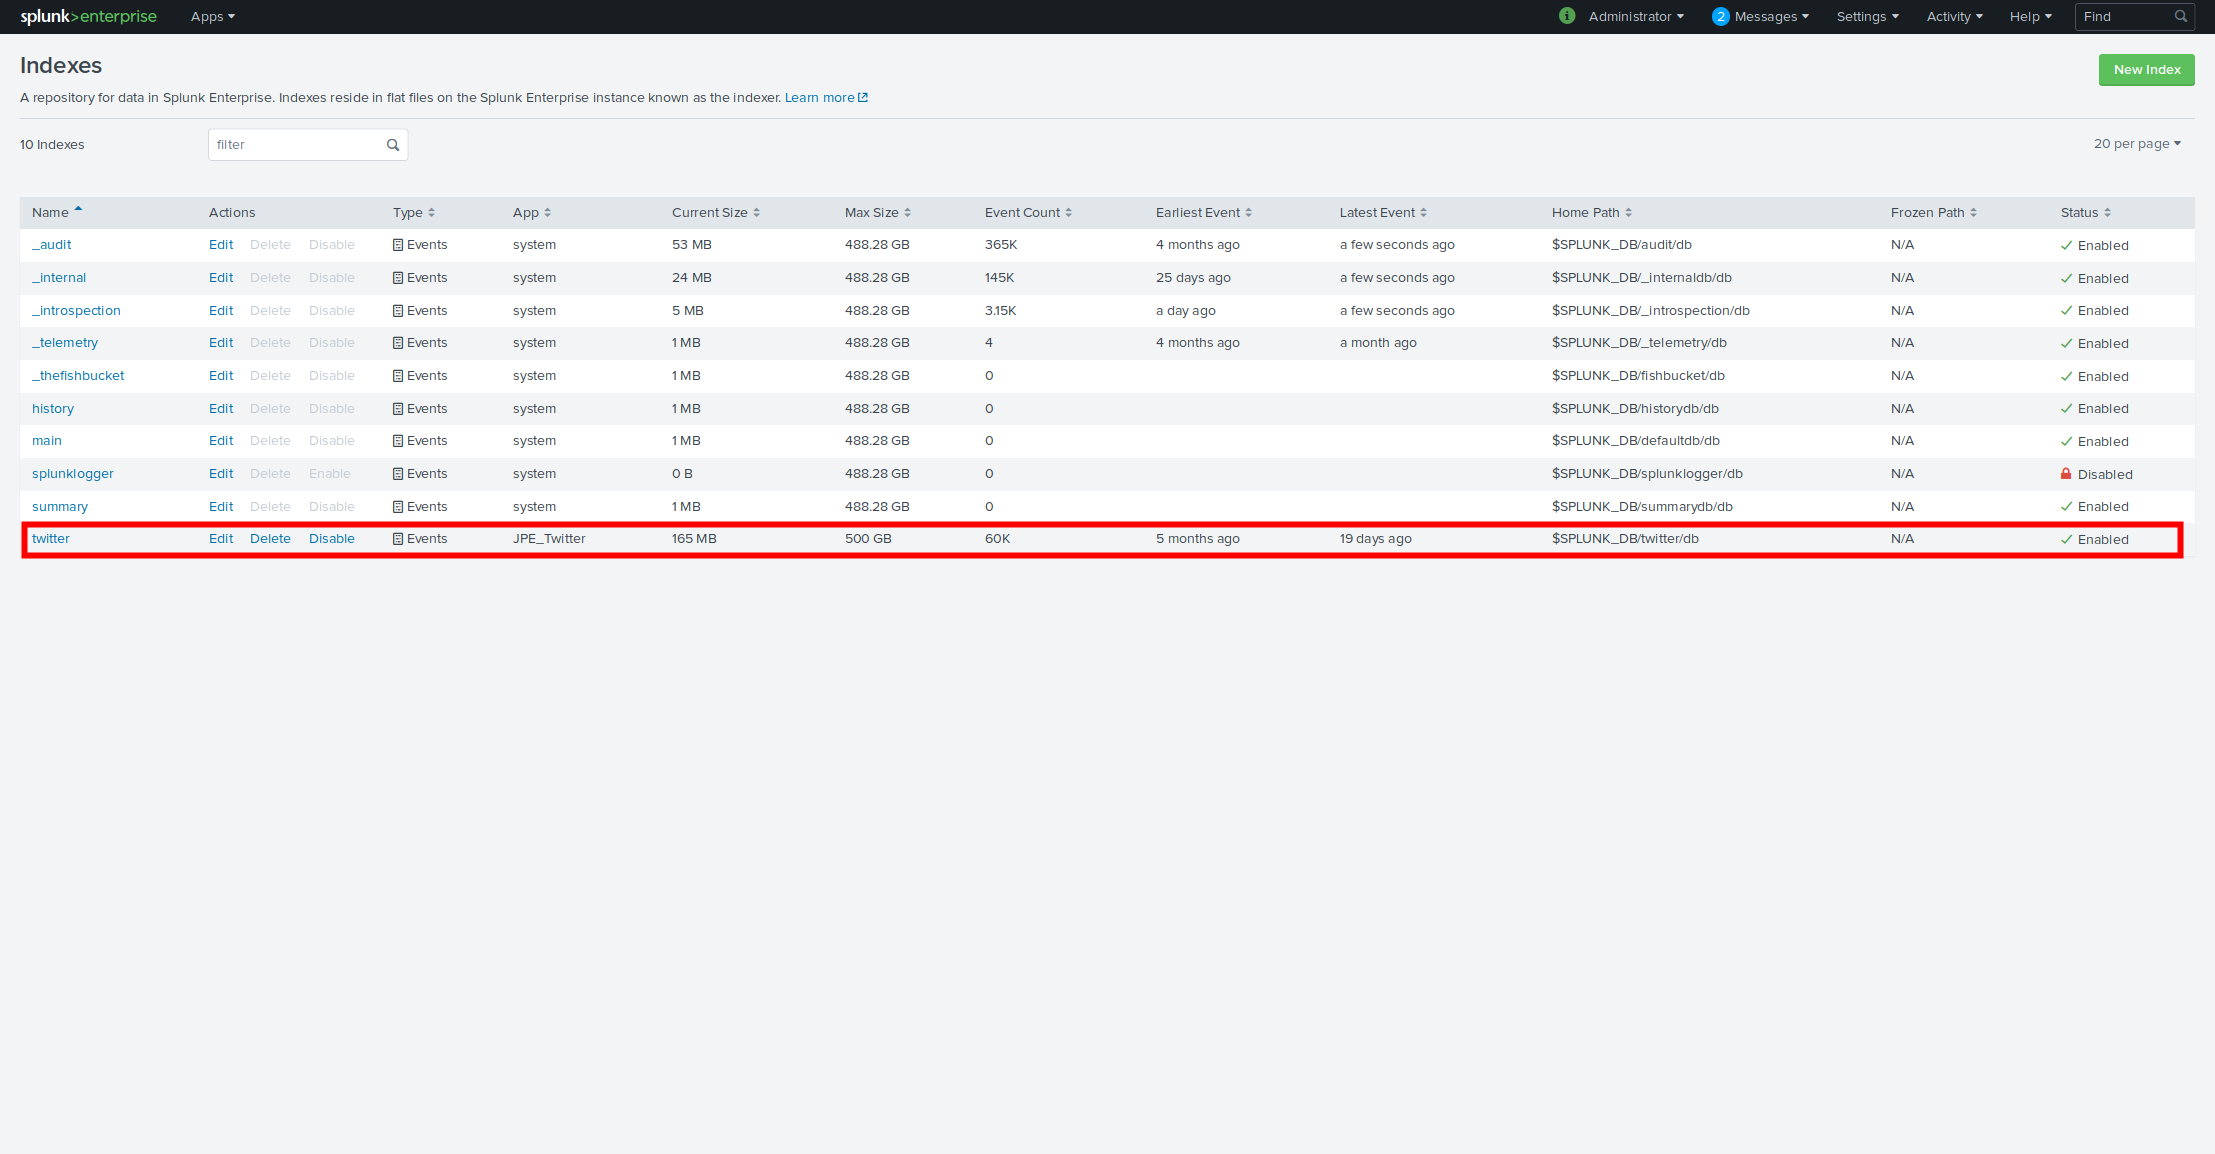
\includegraphics[width=\linewidth]{img/d.png}
    \caption{\color{text} Index}
  \end{subfigure}
  \begin{subfigure}[b]{0.49\linewidth}
    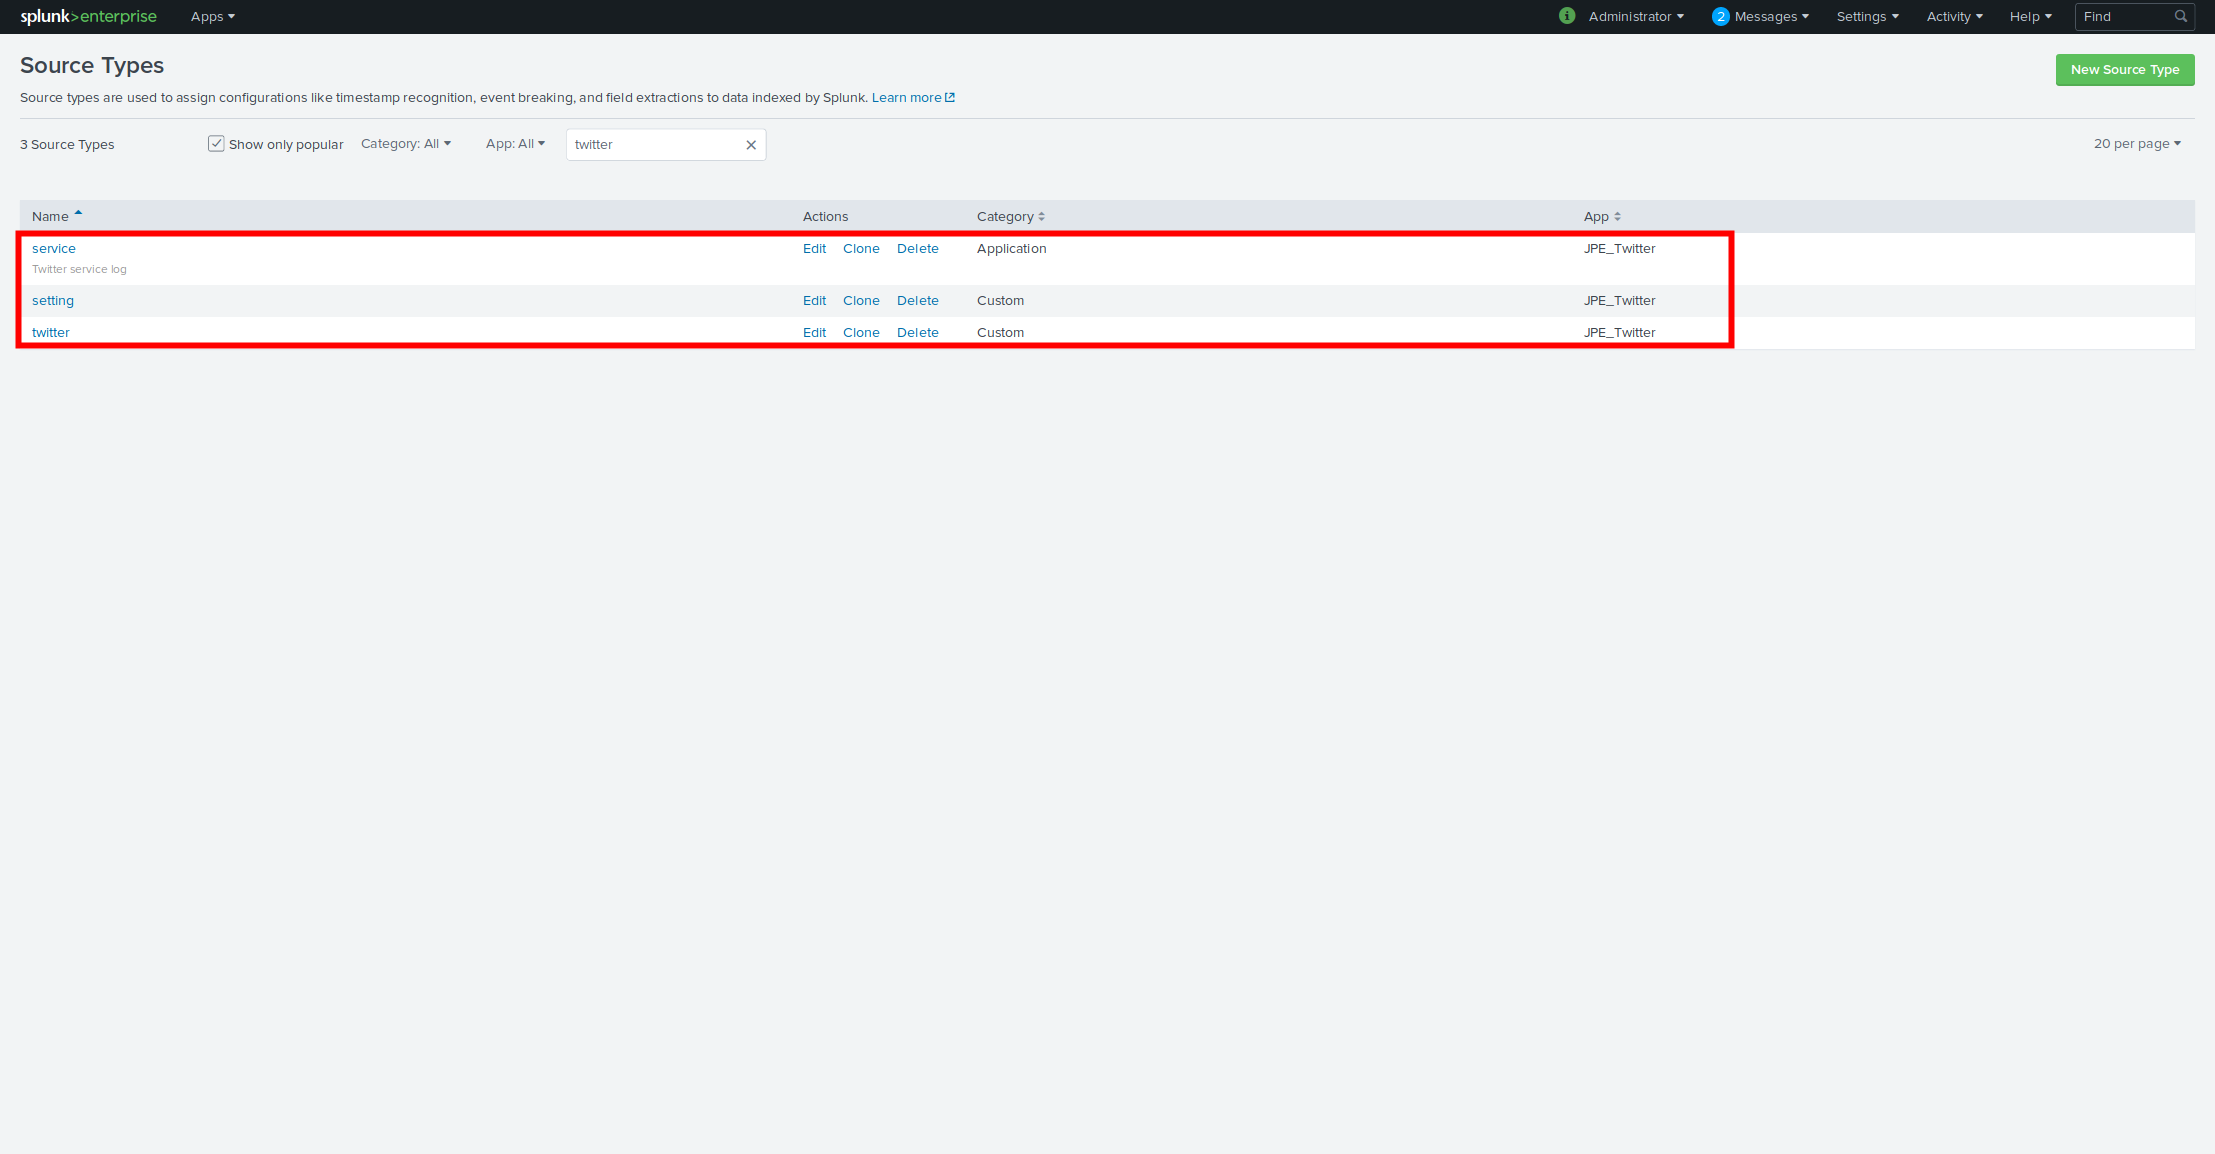
\includegraphics[width=\linewidth]{img/e.png}
    \caption{\color{text} Sourcetype}
  \end{subfigure}
  \caption{\color{text} Validations}
  \label{fig:validacion}
\end{figure}

\textbf{Index twitter: }Data repository of installed application.\\
\textbf{Source Type twitter: }Identify the structure of the filtered data on twitter.\\
\textbf{Source Type service: }Identify the structure of the generated data by \textit{service.py} module.\\
\textbf{Source Type setting: }Identify the structure of the generated data by \textit{twitter.py} y \textit{security.py} modules.
\newline
\section{Support, questions and comments}

\textbf{Full Name: }Juan Alejandro P\'erez Chand\'ia\\
\textbf{E-Mail: }jalejandro.ingeniero@gmail.com\\
\textbf{Languages: }Spanish - English
% \end{large}
\end{document}
